%%%%%%%%%%%%%%%%%%%%%%%%%%%%%%%%%%%%%%%%%%%%%%%%%%%%%%%%%%%%%%%%%%%%
\section{Cryogenics Instrumentation}
\label{sec:fdsp-cryo-instr} % label used for \ref's from single phase sections.
\label{sec:fddp-cryo-instr} % label used for \ref's from dual phase sections.
\label{sec:fdgen-cryo-instr} % label used for \ref's from generic sections.
% Jim G %Carmen

Instrumentation inside the cryostat must ensure that the condition of the \dword{lar} is adequate for operation of the \dshort{tpc}.
This instrumentation includes devices to monitor the impurity level of the argon, e.g., the purity monitors, which provide high precision electron lifetime measurements,
and gas analyzers to ensure that the levels of atmospheric contamination drop below certain limits during the cryostat purging, cooling and filling.
The cryogenics system operation is monitored by temperature sensors deployed in vertical arrays and at the top and bottom of the detector, providing a 
detailed \threed temperature map which can help to predict the \dword{lar} purity across the entire cryostat. The cryogenics instrumentation also includes \lar level monitors and
a system of internal cameras to help in locating sparks in the cryostat and for overall monitoring of the cryostat interior. 
As mentioned in the Introduction, cryogenics instrumentation requires simulation work to identify the proper location for these devices inside the cryostat and
for the coherent analysis of the instrumentation data. 

Figure~\ref{fig:sp-slow-cryo-ports} shows the current map of cryostat ports for the \dword{spmod}, highlighting the ones assigned to instrumentation devices,
as well as the preliminary location for some of these devices. Vertical temperature profilers are located behind the \dwords{apa} ($T_S$) and behind the east end wall ($T_D$).
They are complemented by a coarser \twod grid of sensors at the top and bottom of the cryostat (not shown in the figure). Purity monitors as well as level meters are planned
in each detector side, behind the two front end walls. Inspection cameras will use some of the multipurpose instrumentation ports, but their exact locations are yet to be decided. 

\begin{dunefigure}[Cryostat ports]{fig:sp-slow-cryo-ports}
{Cryostat ports and preliminary location of some instrumentation devices. }
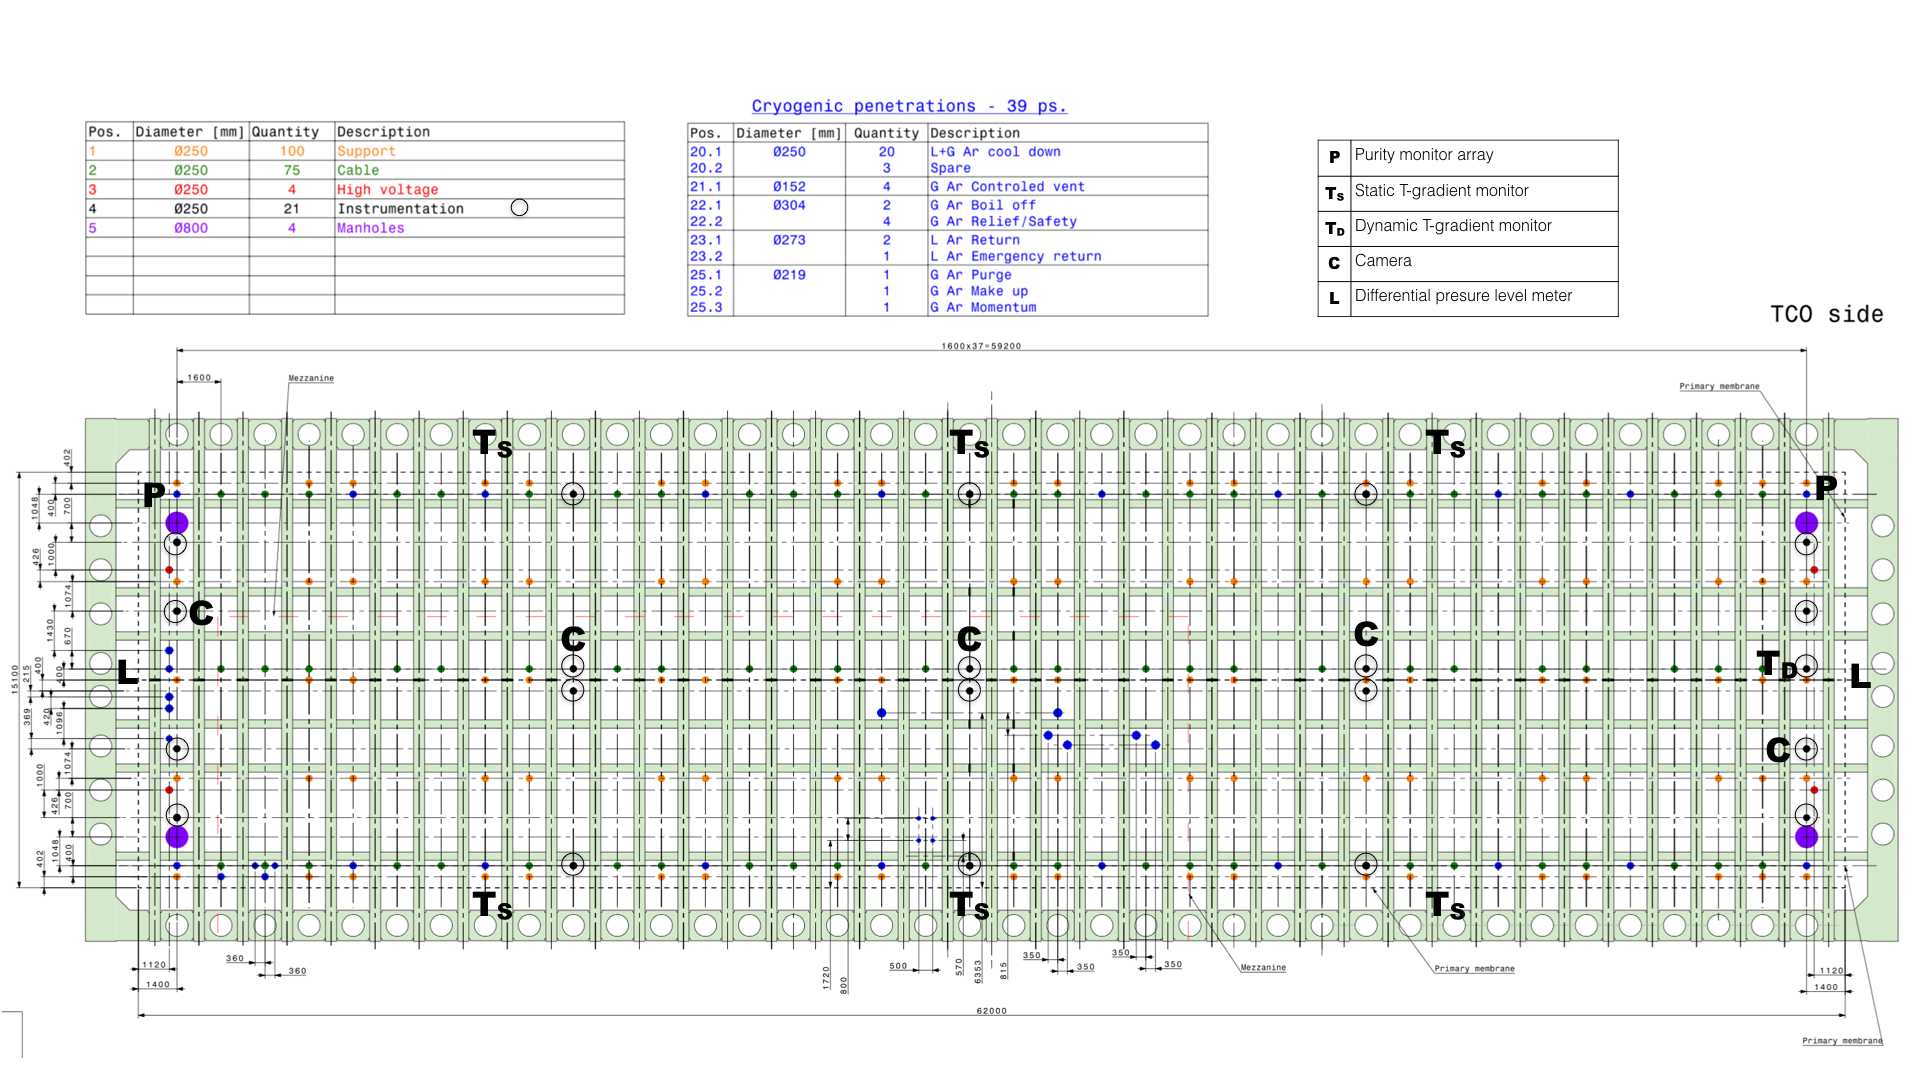
\includegraphics[width=0.95\textwidth]{cisc_cryostat_ports.png}
\end{dunefigure}




%%%%%%%%%%%%%%%%%%%%%%%%%%%%%%%%%%%
\subsection{Fluid Dynamics Simulations}
\label{sec:fdgen-slow-cryo-cfd}
% P. Strons
% S. Gollapinni

Proper placement of purity monitors, thermometers, and liquid level monitors within the \dword{detmodule} requires knowledge of how \dword{lar} behaves within the cryostat in terms of its fluid dynamics, heat and mass transfer, and distribution of impurity concentrations. 
Fluid motion within the cryostat is driven primarily by small changes in density from thermal gradients, although pump flow rates and inlet and outlet locations also contribute. 
Heat sources include exterior heat from the surroundings, interior heat from the electronics, and pump inlet temperature. \fixme{pump inlet temperature per se is not a heat source}

The fluid flow behavior can be determined through simulation of \dword{lar} flow within the detector using ANSYS CFX, a commercially available \dfirst{cfd} code. Such a model must include proper definition of the fluid characteristics, solid bodies and fluid-solid interfaces, and a means for measuring contamination, while still maintaining reasonable solve times.
\fixme{compute times?}
Although simulation of the \dword{detmodule} presents challenges, there exist acceptable simplifications for accurately representing the fluid, the interfacing solid bodies, and variations of contaminant concentrations. Because of the magnitude of thermal variation within the cryostat, modeling of the \dword{lar} is simplified through use of constant thermophysical properties, calculation of buoyant force through use of the Boussinesq Model (using constant a density for the fluid with application of a temperature dependent buoyant force), and a standard shear stress transport turbulence model. Solid bodies that contact the \dword{lar} include the cryostat wall, the cathode planes, the anode planes, the ground plane, and the \dword{fc}. As in previous \dshort{cfd} models of the \dword{35t} cryostat and \dword{protodune} by South Dakota State University (SDSU)~\cite{docdb-5915}, the \dword{fc} planes, anode planes, and \dword{gp} can be represented by porous bodies. Since impurity concentration and electron lifetime do not impact the fluid flow, these variables can be simulated as  passive scalars, as is commonly done for smoke releases~\cite{cfd-1} in air or dyes released in liquids.

\fixme{some of this sounds very SP to me -anne}

Significant discrepancies between real data and simulations can have potential impacts on detector performance, as simulation results contribute to decisions about where to locate sensors and monitors, as well as definitions of various calibration quantities. However, methods of mitigating such risks include well established convergence criteria, sensitivity studies, and comparison to results of previous \dshort{cfd} simulation work by SDSU and \fnal. Additionally, the simulation will be improved with input from temperature measurements and validation tests until the required agreement is achieved.
\fixme{...tests. (anne)}

%%%%% Must find better pictures. Just use this for now %%% anne to here Fri 4/27
\begin{dunefigure}[\dshort{cfd} example]{fig:cfd-example}
  {Distribution of temperature on a plane intersecting an inlet (right) and halfway between an inlet and an outlet (left), as predicted by SDSU \dshort{cfd} simulations \cite{docdb-5915}. (See Figure\ \ref{fig:cfd-example-geometry} for geometry.)}
  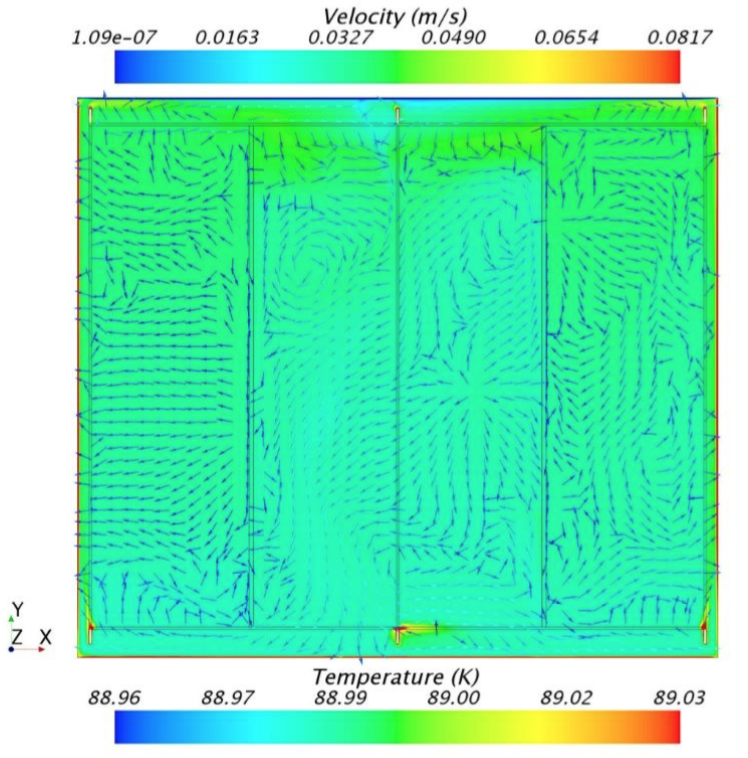
\includegraphics[height=0.4\textwidth]{cisc_cfd_outlet_z0.png}
  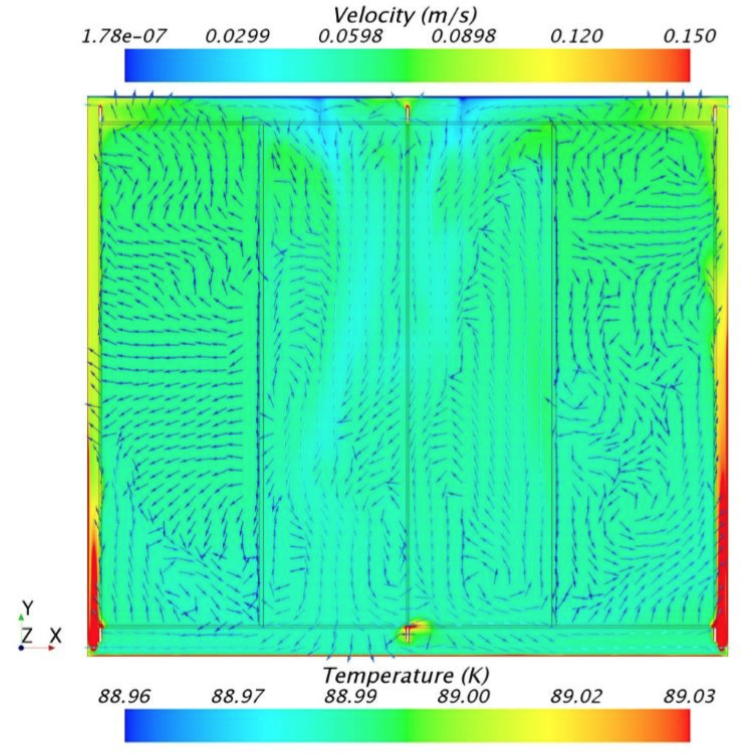
\includegraphics[height=0.4\textwidth]{cisc_cfd_inlet_z52.png}
\end{dunefigure}

Figure~ref{fig:cfd-example} shows an example of the temperature
distribution on a plane intersecting a \dword{lar} inlet and at a
plane halfway between an inlet and an outlet; the geometry used for
this simulation is shown in Figure\ \ref{fig:cfd-example-geometry}.
Note the plume of higher temperature \dword{lar} between the walls and
the outer APA on the inlet plane.  The current locations of instrumentation in
the cryostat as shown in Figure~ref{fig:sp-slow-cryo-ports} were
determined using the temperature and impurity distributions from these
previous simulations.

\begin{dunefigure}[\dshort{cfd} example geometry]{fig:cfd-example-geometry}
  {Layout of the \dshort{tpc} within the cryostat (top) and positions of
    \dword{lar} inlets and outlets (bottom) as modeled in the SDSU
    \dshort{cfd} simulations \cite{docdb-5915}.
    The Y axis is vertical and the X axis is parallel to the \dword{tpc}
    drift direction.
    Inlets are shown in green and outlets are shown in red.}
  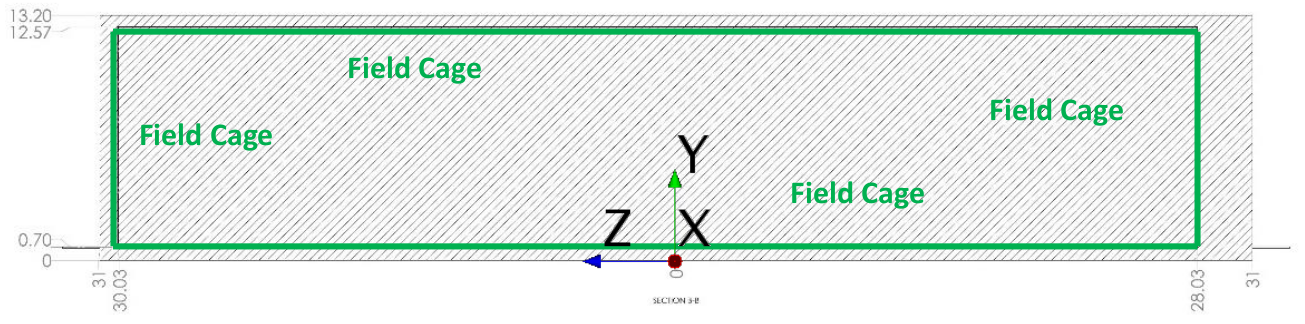
\includegraphics[width=0.8\textwidth]{cisc_cfd_cryostat-layout}
  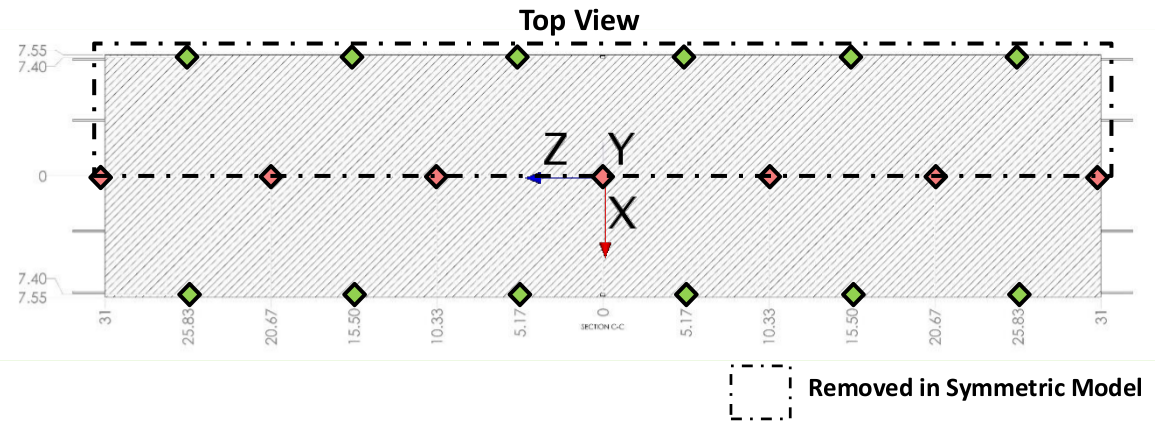
\includegraphics[width=0.8\textwidth]{cisc_cfd_inlet-outlet-layout}
\end{dunefigure}

The initial strategy for the future \dword{cfd} simulation effort is to understand the performance of \dword{protodune} cryogenics system and model the \dwords{fd} to derive requirements for instrumentation devices.
The following is a prioritized set of studies planned to help drive the requirements for other systems:
\begin{enumerate}
\item Review the DUNE \dword{fd} cryogenics system design and verify the current implementation in simulation; this is important to ensure that the model represents what will be built.
\item Model the \dword{pddp}  liquid and gas regions with the same precision as the \dword{fd}; presently only liquid model exists; the liquid model is needed to interpret the thermometer data and the gas model is needed to understand how to place thermometers in the ullage and verify the design of gaseous argon purge system.
\item Perform a \dword{cfd} study to determine the feasibility of a wier for \dual; this helps to determine if it can be used to clean the \lar surface before the extraction grid is submerged in the \dword{dpmod}.
\item Verify the \dword{spmod} \single \dword{cfd} model in simulation performed by LBNF; this defines the requirements for instrumentation devices (e.g., thermometry).
\item Model the \dword{pddp} liquid and gas regions with the same precision as the \dword{fd}. \fixme{same as a previous bullet}
\end{enumerate}